% ::setlocal makeprg=cd\ latex\ &&\ pdflatex\ -interaction=batchmode\ main.tex\ &&\ xdg-open\ main.pdf\ &&\ exit
\chapter{Beautiful Closed Orbits}
\label{app:beautiful}

Once the integral of the precession has been expressed in terms of elliptic
integrals (eq. \ref{cap2:eq:delta_phi_elliptic}), we can use a numerical method
to find the values of $\hat \ell$ and $\mathcal E$ that gives a desired
precession angle $\delta \phi$.
Figure \ref{app:fig:prec_theory} shows $\delta \phi (\mathcal E)$ for some of
the possible values of $\hat \ell$, allowing us to reduce the problem to one
dimension, where we can use the bisection method to find $\mathcal E$.

\begin{figure}[h]
    \centering
    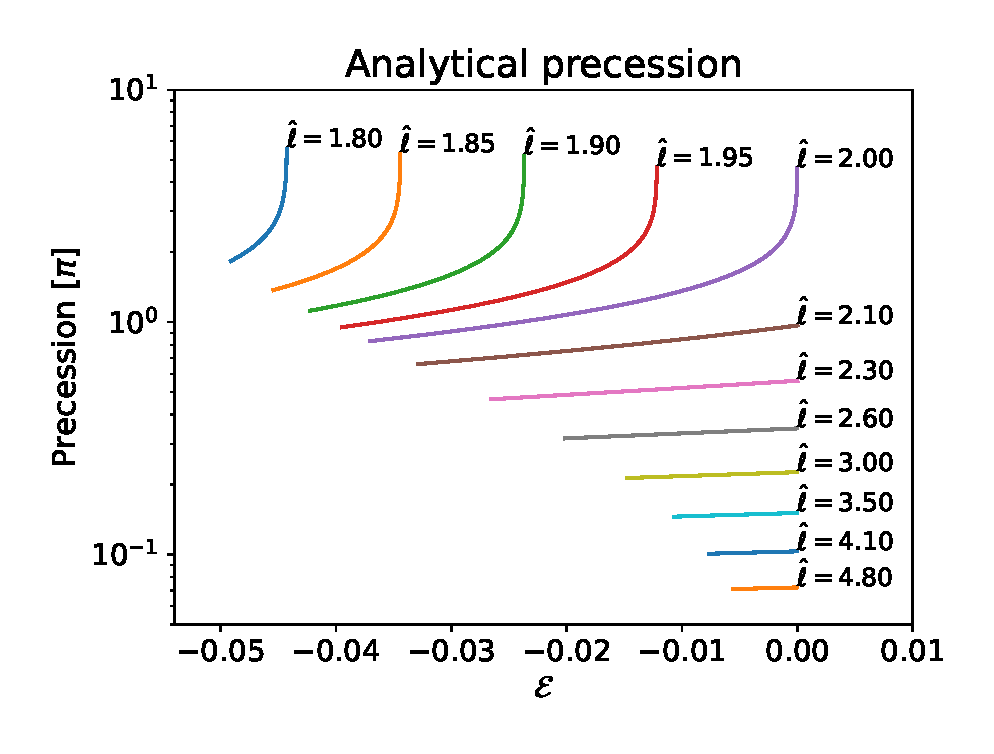
\includegraphics[width=0.7\textwidth]{Figures/chapter2/prec_theory.eps}
    \caption{Precession angle as a function of $\mathcal E$, different values
    of $\hat \ell$ are shown. \\
    For each value of $\hat \ell$ the energy ranges from $V_{\rm min} + 
    \num{1e-8}$ to $\min{(V_{\rm max}, ~0)}$.}
    \label{app:fig:prec_theory}
\end{figure}

It is now possible to find orbits with exactly $\delta \phi = 2 \pi / n$,
where $n \in \mathbb{N}$.
These orbits will pass through the same point in the $x-y$ plane after $n$
revolutions.

Figures \ref{appB:fig:n2} to \ref{appB:fig:n20}
show some of the closed orbits found using this method.
Figure \ref{appB:fig:n20_err} also provides another test of the numerical
stability of the method.

The program that implements the numerical method described in section
\ref{cap2:sec:alt_method} and generates the data shown in the figures is
\texttt{main.x}
\footnote{The source code is available at
\url{https://github.com/F-Depi/geodetiche-metrica-Schwarzschild}.}
and the argument needed are specified in Table \ref{app:tab:code}.

\begin{table}[h]
    \centering
    \begin{tabular}{|l|l|}
        \hline
        \texttt{./main.x 2 -0.0240788493 -t 1000 -a 1 -r 1000} & \ref{appB:fig:n2} \\
        \texttt{./main.x 2.2 -0.0055406976 -t 1e4 -a 1 -r 1000} & \ref{appB:fig:n3} \\
        \texttt{./main.x 2.33 -0.0079962099 -t 1e4 -a 1 -r 1000} & \ref{appB:fig:n4} \\
        \texttt{./main.x 3.12 -0.0041308673 -t 1e5 -a 1 -r 1000 -h 0.01 -B 5} & \ref{appB:fig:n10} \\
        \texttt{./main.x 4.12 -0.0064453981 -t 1e5 -a 1 -r 1000 -h 0.01 -B 5} & \ref{appB:fig:n20} \\
        \texttt{./main.x 4.12 -0.0064453981 -t 1e5 -a 1 -r 1000 -h 0.01 -B 50} & \ref{appB:fig:n20_err} \\
        \hline
    \end{tabular}
    \caption{Code used to generate the data for the figures.}
    \label{app:tab:code}
\end{table}

\begin{figure}[h!]
    \begin{minipage}{0.49\textwidth}
        \centering
        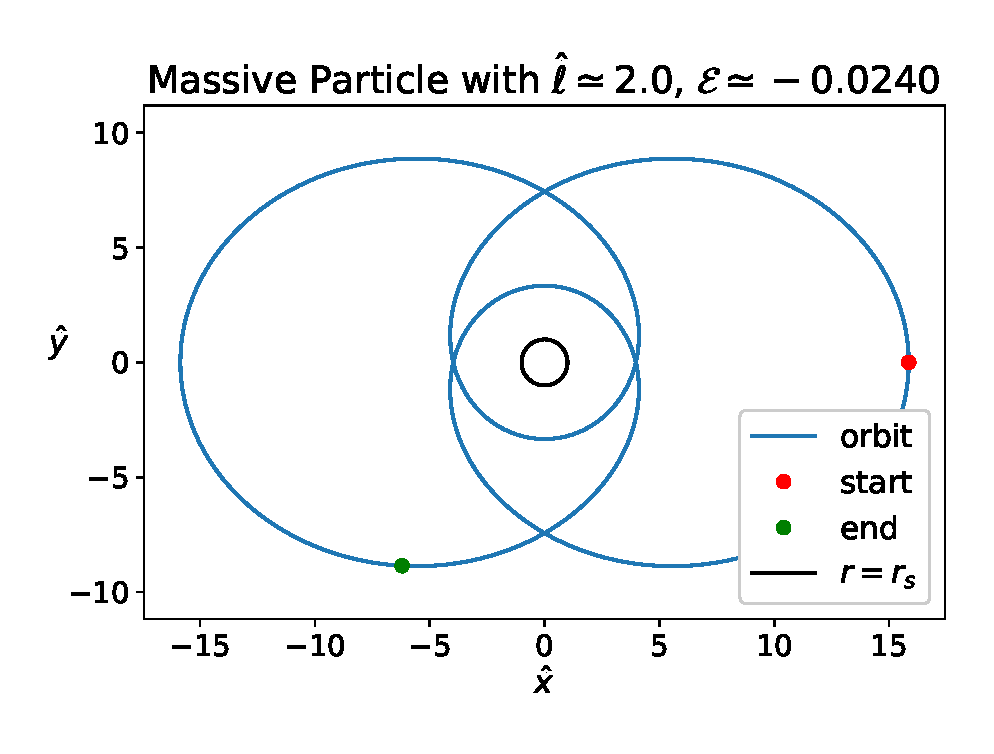
\includegraphics[width=\textwidth]{Figures/appendixB/beautiful2.eps}
        \caption{$\hat \ell = 2, ~ \mathcal E =  -0.0240788493$, \\
        $\delta \phi = \pi$}
        \label{appB:fig:n2}
    \end{minipage}
    \hspace{0.01\textwidth}
    \begin{minipage}{0.49\textwidth}
        \centering
        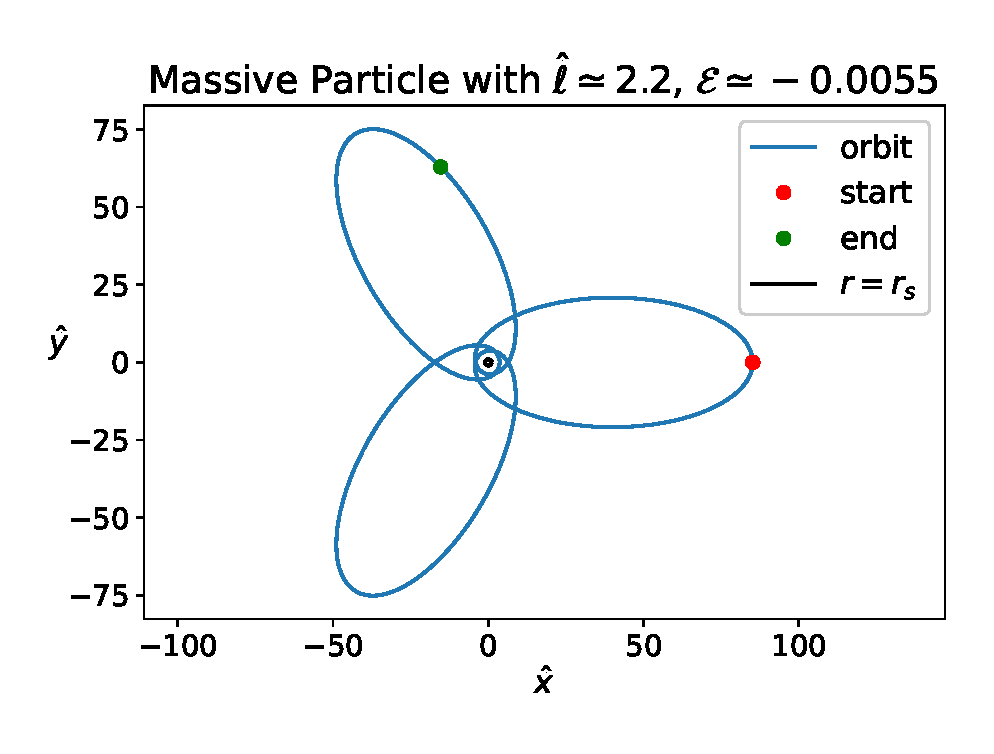
\includegraphics[width=\textwidth]{Figures/appendixB/beautiful3.eps}
        \caption{$\hat \ell = 2.2, ~ \mathcal E = -0.0055406976$ \\
        $\delta \phi = 2 \pi / 3$}
        \label{appB:fig:n3}
    \end{minipage}
\end{figure}


\begin{figure}[h!]
    \begin{minipage}{0.49\textwidth}
        \centering
        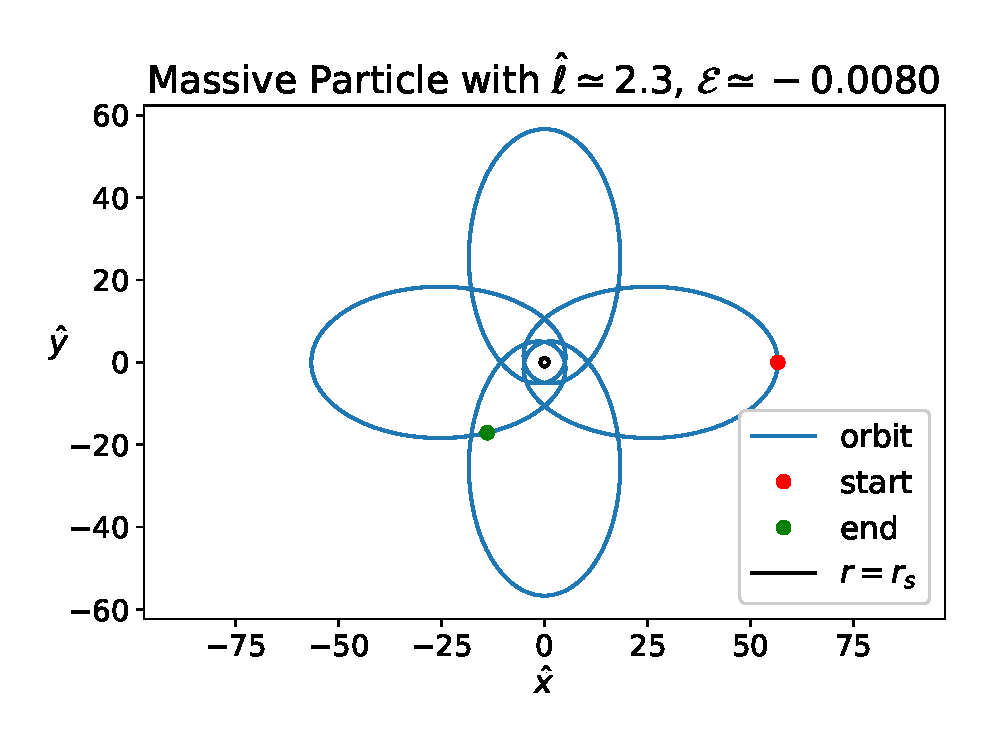
\includegraphics[width=\textwidth]{Figures/appendixB/beautiful4.eps}
        \caption{$\hat \ell = 2.33, ~ \mathcal E = -0.0079962099$, \\
        $\delta \phi = \pi / 2$}
        \label{appB:fig:n4}
    \end{minipage}
    \hspace{0.01\textwidth}
    \begin{minipage}{0.49\textwidth}
        \centering
        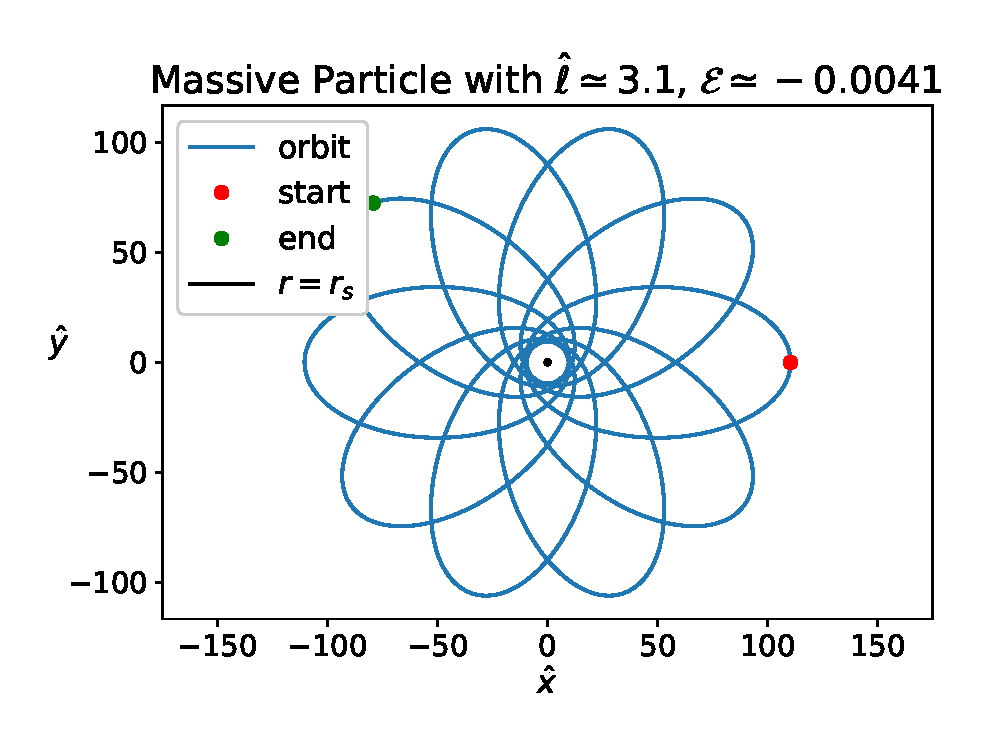
\includegraphics[width=\textwidth]{Figures/appendixB/beautiful10.eps}
        \caption{$\hat \ell = 3.12, ~ \mathcal E = -0.0041308673$, \\
        $\delta \phi = \pi / 5$}
        \label{appB:fig:n10}
    \end{minipage}
\end{figure}


\begin{figure}[h!]
    \begin{minipage}{0.49\textwidth}
        \centering
        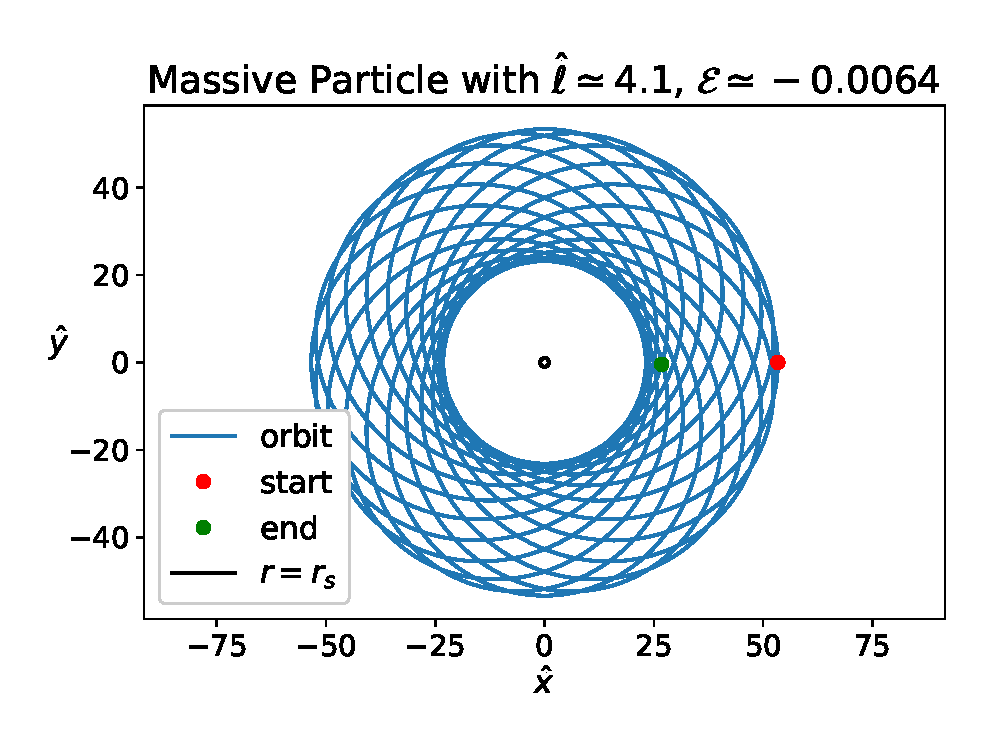
\includegraphics[width=\textwidth]{Figures/appendixB/beautiful20.eps}
        \caption{$\hat \ell = 4.12, ~ \mathcal E = -0.0064453981$, \\
        $\delta \phi = \pi / 10$ \\ \\ \\}
        \label{appB:fig:n20}
    \end{minipage}
    \hspace{0.01\textwidth}
    \begin{minipage}{0.49\textwidth}
        \centering
        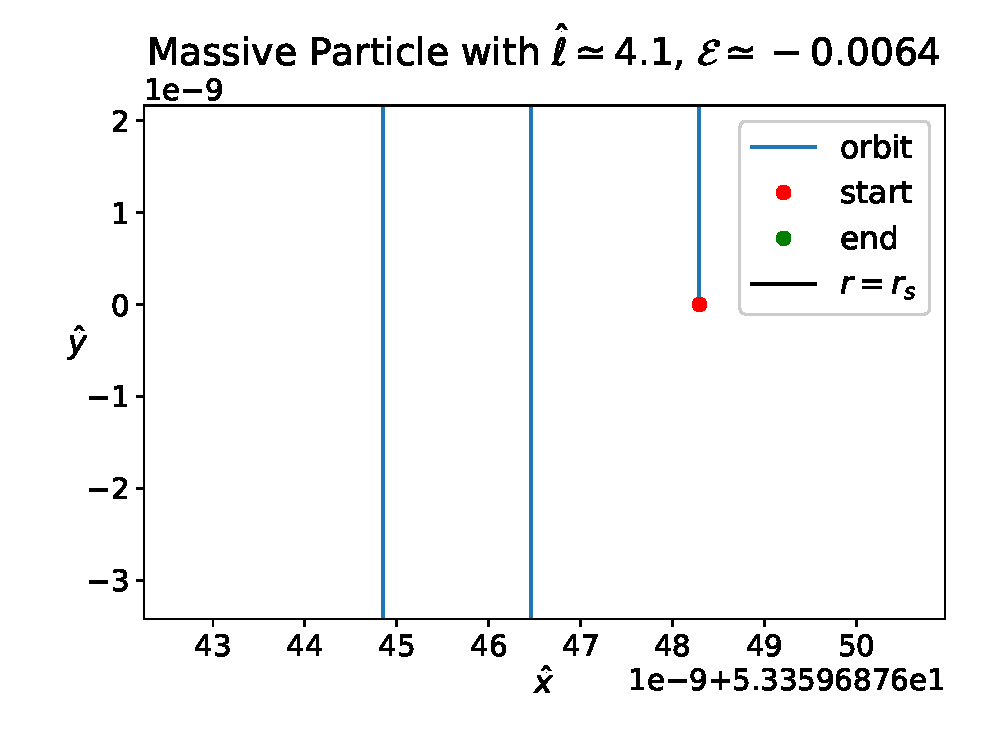
\includegraphics[width=\textwidth]{Figures/appendixB/beautiful20_err.eps}
        \caption{Zoom on the starting point area of figure \ref{appB:fig:n20}.
        As expected from the numerical approximation the particle does not
        return to the same exact point, the error is $\sim 10^{-9}$ with $h = 0.01$.}
        \label{appB:fig:n20_err}
    \end{minipage}
\end{figure}

\begin{figure}[h!]
    \centering
    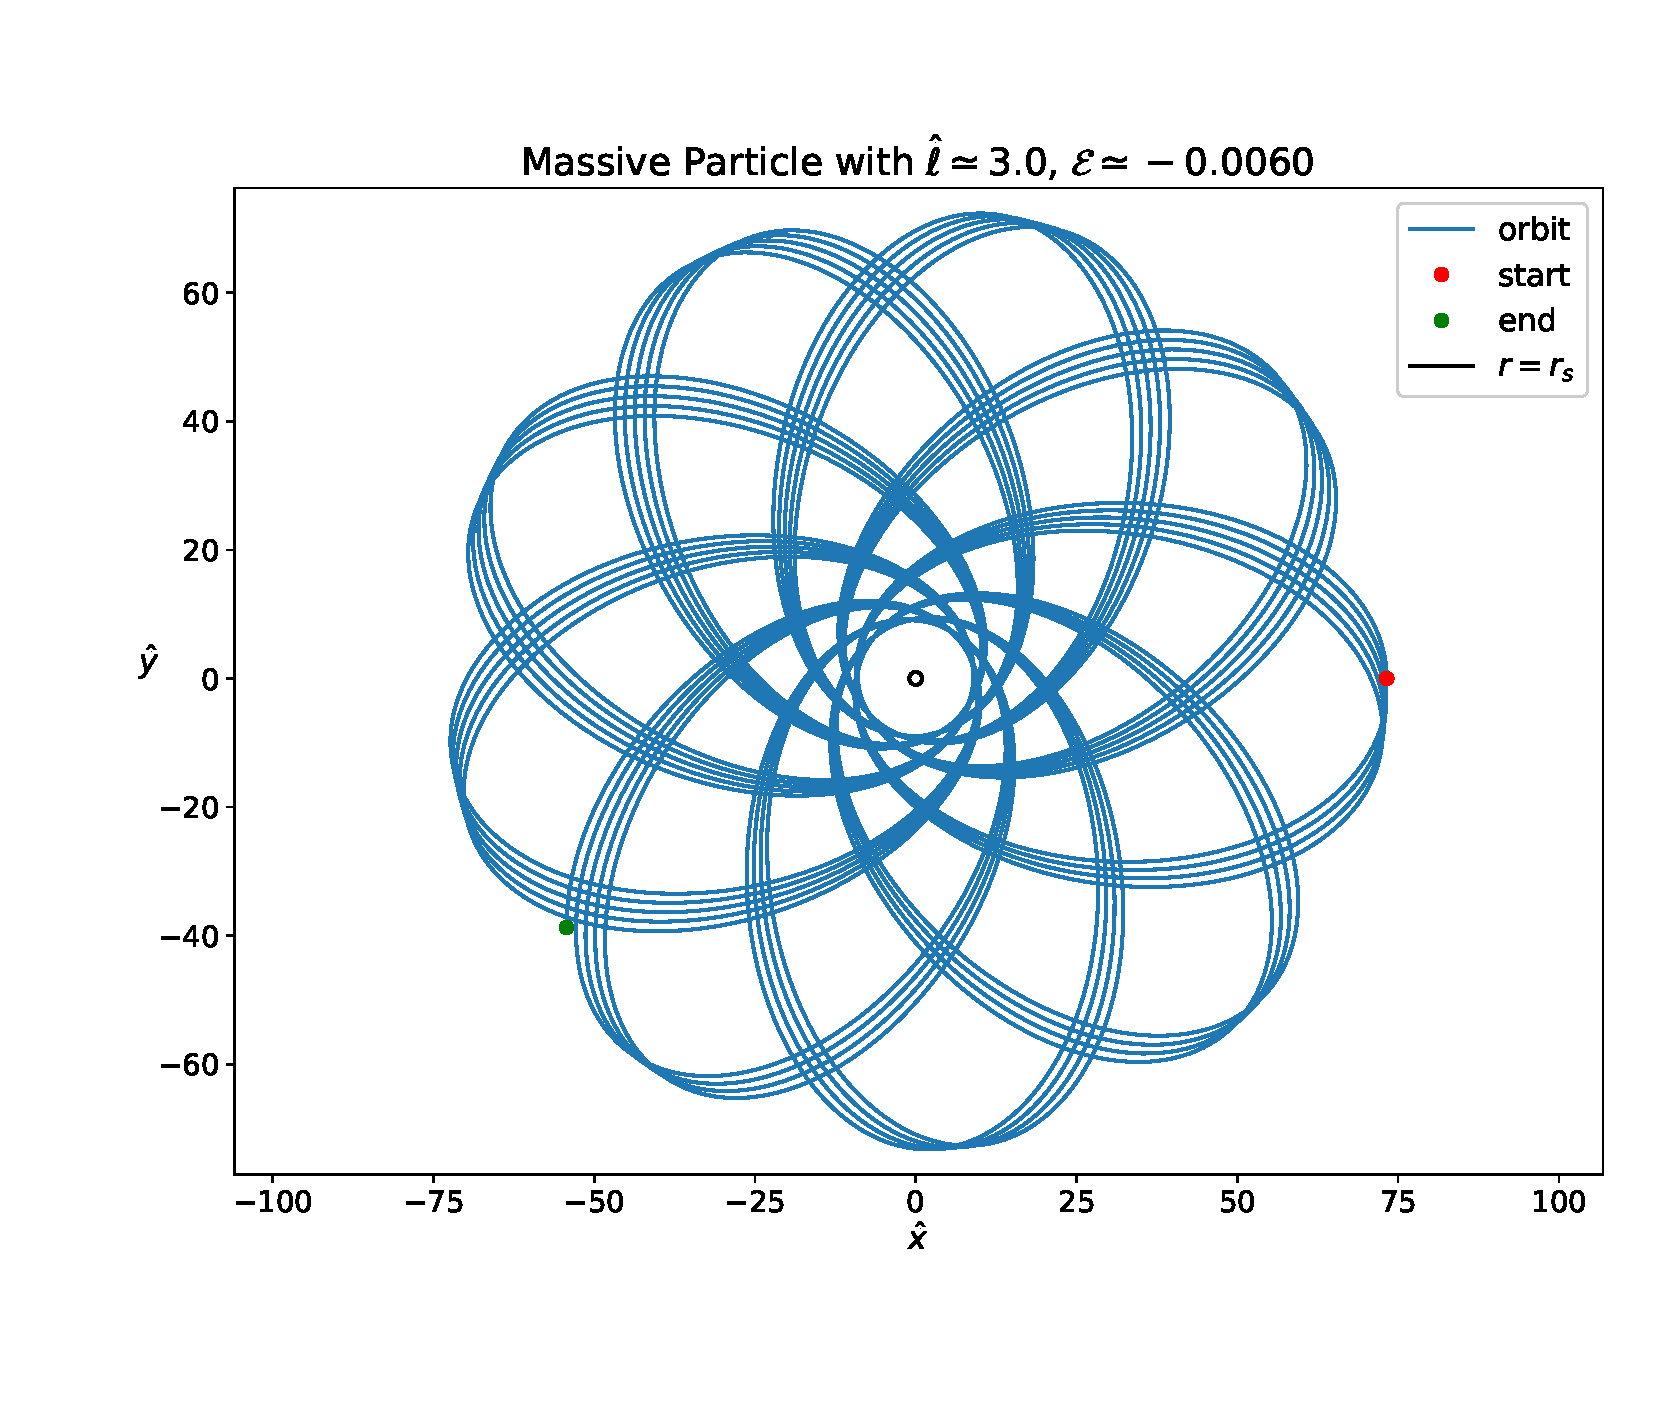
\includegraphics[width=0.85 \textwidth]{Figures/appendixB/spirograph.eps}
    \caption{$\hat \ell = 3, ~ \mathcal E = -0.006, ~ \delta \phi \simeq 0.221
    \pi$.
    We don't know if the particle will ever return to the starting point as the
    theoretical precession is evaluated numerically and could be an irrational
    number.}
    \label{appB:fig:spirograph}
\end{figure}
